\documentclass[polish,a4paper]{article}
\usepackage[T1]{fontenc}
\usepackage[utf8]{inputenc}
\usepackage{babel}
\usepackage{pslatex}
\usepackage{pgfplots}
\usepackage{circuitikz} 
\usetikzlibrary{circuits.ee.IEC}
\usepackage{anysize}
\marginsize{2.5cm}{2.5cm}{3cm}{3cm}

%rysunek obwodu - EWA
%\tikzset{circuit declare symbol = AC source}
%\tikzset{AC source IEC graphic/.style={
%    circuit symbol lines,
%    circuit symbol size=width 2 height 2,
%    shape=generic circle IEC,
%    /pgf/generic circle IEC/before background={
%    \pgfpathmoveto{\pgfpoint{-0.8pt}{0pt}}
%    \pgfpathsine{\pgfpoint{0.4pt}{0.4pt}}
%    \pgfpathcosine{\pgfpoint{0.4pt}{-0.4pt}}
%    \pgfpathsine{\pgfpoint{0.4pt}{-0.4pt}}
%    \pgfpathcosine{\pgfpoint{0.4pt}{0.4pt}}
%    \pgfusepath{stroke}
%    },
%    transform shape, draw
%  }
%}
%\tikzset{circuit ee IEC/.append style=
%  {set AC source graphic = AC source IEC graphic}
%}

%\begin{figure}[!h]

%\centering
%\begin{tikzpicture}[
%    circuit ee IEC,
%    x = 1.5cm, y = 1cm,
%    every info/.style = {font = \scriptsize},
%    set diode graphic = var diode IEC graphic,
%    set make contact graphic = var make contact IEC graphic,
%  ]

%\draw (0,-2) to [vco] (0,2) --
%	  (0,2) to [capacitor={farad=10n,info'={$C$}}] (2,2) --   
%      (2,2) to [inductor={henry=66m,info'={$L$}}] (4,2) --
%      (4,2) to [resistor={ohm=1k,info'={$R$}}] (4,-2) --
%      (4,-2) to [resistor={ohm=2k,info'={$R$}}] (3,-2) --
%      (3,-2) to (3,-1) --
%      (3,-1) to [resistor={ohm=2k,info'={$R$}}] (1,-1) --
%      (1,-1) to (1,-2)
%      (3,-2) to (3,-3) --
%      (3,-3) to [resistor={ohm=2k,info'={$R$}}] (1,-3) --
%      (1,-3) to (1,-2) --
%      (1,-2) to (0,-2);
     
      

%\end{tikzpicture}
%\caption{Badany obwód RLC}
%\label{fig:rlc}
%\vspace{2cm}

%\begin{figure}[!h]
%\centering
%\begin{tikzpicture}[
%    circuit ee IEC,
%    x = 2cm, y = 1cm,
%    every info/.style = {font = \scriptsize},
%    set diode graphic = var diode IEC graphic,
%    set make contact graphic = var make contact IEC graphic,
%  ]

%\draw (0,0) to [resistor={info'={$R3$}}] (1,0) --
%	  (1,0) to (1,-1) --
%	  (1,-1) to [resistor={info'={$R4$}}] (3.25,-1)
%	  (1,0) to (1,1) --
%	  (1,1) to (1.25,1) --
%	  (1.25,1) to (1.25,1.5) --
%	  (1.25,1.5) to [resistor={info'={$R1$}}] (2.25,1.5) --
%	  (2.25,1.5) to (2.25,1)
%	  (1.25,1) to (1.25,0.5) --
%	  (1.25,0.5) to [resistor={info'={$R2$}}] (2.25,0.5) --
%	  (2.25,0.5) to (2.25,1)
%	  (2.25,1) to [resistor={info'={$R5$}}] (3.25,1) --
%	  (3.25,1) to (3.25,0)
%	  (3.25,-1) to (3.25,0)--
%	  (3.25,0) to (3.75,0);
%\path (-0.3,0) node(x) {{A}}
%	  (4.05,0) node(x) {{B}};
%\end{tikzpicture}
%\end{figure}

\begin{document}
Zadanie B, część I
\begin{figure}[!h]
\centering
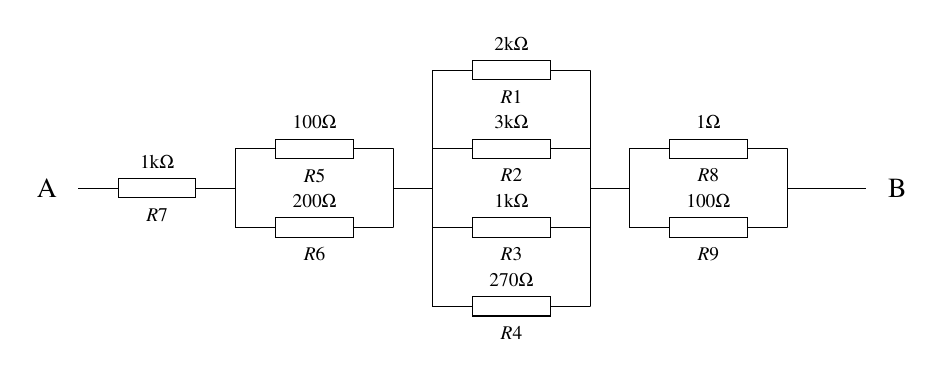
\begin{tikzpicture}[
    circuit ee IEC,
    x = 2cm, y = 1cm,
    every info/.style = {font = \scriptsize},
    set diode graphic = var diode IEC graphic,
    set make contact graphic = var make contact IEC graphic]

\draw (0,0) to [resistor={ohm=1k, info'={$R7$}}] (1,0) --
	  (1,0) to (1,0.5)--
	  (1,0.5) to [resistor={ohm=100, info'={$R5$}}] (2,0.5) --
	  (2,0.5) to (2,0)
	  (1,0) to (1,-0.5)--
	  (1,-0.5) to [resistor={ohm=200, info'={$R6$}}] (2,-0.5) --
	  (2,-0.5) to (2,0)--
	  (2,0) to (2.25,0)--
	  (2.25,0) to (2.25,1.5)--
	  (2.25,1.5) to [resistor={ohm=2k, info'={$R1$}}] (3.25,1.5) --
	  (3.25,1.5) to (3.25,0)
	  (2.25,0) to (2.25,-1.5)--
	  (2.25,-1.5) to [resistor={ohm=270, info'={$R4$}}] (3.25,-1.5) --
	  (3.25,-1.5) to (3.25,0)
	  (2.25,-0.5) to [resistor={ohm=1k, info'={$R3$}}] (3.25,-0.5)
	  (2.25,0.5) to [resistor={ohm=3k, info'={$R2$}}] (3.25,0.5)
	  (3.25,0) to (3.5,0) --
	  (3.5,0) to (3.5,0.5) --
	  (3.5, 0.5) to [resistor={ohm=1, info'={$R8$}}] (4.5, 0.5) --
	  (4.5, 0.5) to (4.5,0)
	  (3.5,0) to (3.5,-0.5) --
	  (3.5,-0.5) to [resistor={ohm=100, info'={$R9$}}] (4.5,-0.5) --
	  (4.5,-0.5) to (4.5,0) --
	  (4.5,0) to (5,0);  
\path (-0.2,0) node(x) {{A}}
	  (5.2,0) node(x) {{B}};
\end{tikzpicture}
\end{figure}
\newline






Zadanie B, część II, obwód 1
\begin{figure}[!h]
\centering
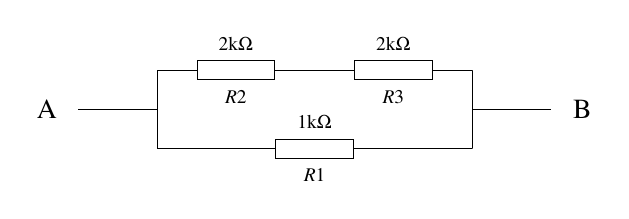
\begin{tikzpicture}[
    circuit ee IEC,
    x = 2cm, y = 1cm,
    every info/.style = {font = \scriptsize},
    set diode graphic = var diode IEC graphic,
    set make contact graphic = var make contact IEC graphic]

\draw (0,0) to (0.5,0) --
	  (0.5,0) to (0.5,0.5)--
	  (0.5,0.5) to [resistor={ohm=2k, info'={$R2$}}] (1.5,0.5) --
	  (1.5,0.5) to [resistor={ohm=2k, info'={$R3$}}] (2.5, 0.5) -- 
	  (2.5,0.5) to (2.5,0)
	  (0.5,0) to (0.5,-0.5)--
	  (0.5,-0.5) to [resistor={ohm=1k, info'={$R1$}}] (2.5,-0.5) --
	  (2.5,-0.5) to (2.5,0) --
	  (2.5,0) to (3,0); 
\path (-0.2,0) node(x) {{A}}
	  (3.2,0) node(x) {{B}};
\end{tikzpicture}
\end{figure}
\newline

Zadanie B, część II, obwód 2
\begin{figure}[!h]
\centering
\begin{tikzpicture}[
    circuit ee IEC,
    x = 2cm, y = 1cm,
    every info/.style = {font = \scriptsize},
    set diode graphic = var diode IEC graphic,
    set make contact graphic = var make contact IEC graphic]

\draw (0,0) to (0.5,0) --
	  (0.5,0) to (0.5,-0.5) --
	  (0.5,-0.5) to [resistor={ohm=100, info'={$R4$}}] (3.75,-0.5) --
	  (3.75,-0.5) to (3.75, 0)
	  (0.5,0) to (0.5,1) --
	  (0.5,1) to (0.75,1) --
	  (0.75,1) to (0.75,1.5) --
	  (0.75,1.5) to [resistor={ohm=1k, info'={$R1$}}] (1.75,1.5) --
	  (1.75,1.5) to (1.75,1)
	  (0.75,1) to (0.75,0.5) --
	  (0.75,0.5) to [resistor={ohm=2k, info'={$R2$}}] (1.75,0.5) --
	  (1.75,0.5) to (1.75,1) --
	  (1.75,1) to [resistor={ohm=1k, info'={$R3$}}] (2.75,1) --
	  (2.75,1) to [resistor={ohm=100, info'={$R5$}}] (3.75,1) --
	  (3.75,1) to (3.75,0)--
	  (3.75,0) to (4.25,0);
\path (-0.2,0) node(x) {{A}}
	  (4.45,0) node(x) {{B}};
\end{tikzpicture}
\end{figure}
\newline

Zadanie B, część II, obwód 3
\begin{figure}[!h]
\centering
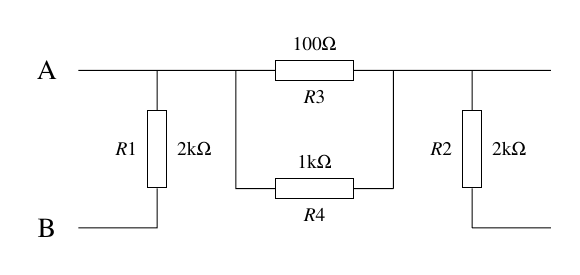
\begin{tikzpicture}[
    circuit ee IEC,
    x = 2cm, y = 1cm,
    every info/.style = {font = \scriptsize},
    set diode graphic = var diode IEC graphic,
    set make contact graphic = var make contact IEC graphic]

\draw (0,0) to (0.5,0) --
	  (0.5,0) to [resistor={ohm=2k, info'={$R1$}}] (0.5,-2) --
	  (0.5,-2) to (0, -2)
	  (0.5,0) to (1,0) --
	  (1,0) to [resistor={ohm=100, info'={$R3$}}] (2,0)
	  (1,0) to (1,-1.5) --
	  (1,-1.5) to [resistor={ohm=1k, info'={$R4$}}] (2,-1.5)--
	  (2,-1.5) to (2,0) --
	  (2,0) to (2.5,0) --
	  (2.5,0) to [resistor={ohm=2k, info'={$R2$}}] (2.5, -2) --
	  (2.5,-2) to (3,-2)
	  (2.5,0) to (3,0) ;
\path (-0.2,0) node(x) {{A}}
	  (-0.2,-2) node(x) {{B}};
\end{tikzpicture}
\end{figure}
\newpage

Zadanie B, część II, obwód 4
\begin{figure}[!h]
\centering
\begin{tikzpicture}[
    circuit ee IEC,
    x = 2cm, y = 1cm,
    every info/.style = {font = \scriptsize},
    set diode graphic = var diode IEC graphic,
    set make contact graphic = var make contact IEC graphic]

\draw (0,0) to (0.5,0) --
	  (0.5,0) to (0.5,-0.5) --
	  (0.5,-0.5) to [resistor={ohm=1k, info'={$R4$}}] (3.75,-0.5) --
	  (3.75,-0.5) to (3.75, 0)
	  (0.5,0) to (0.5,1) --
	  (0.5,1) to (0.75,1) --
	  (0.75,1) to (0.75,1.5) --
	  (0.75,1.5) to [resistor={ohm=100, info'={$R5$}}] (1.75,1.5) --
	  (1.75,1.5) to [resistor={ohm=1k, info'={$R1$}}] (2.75,1.5) --
	  (2.75,1.5) to (2.75,1)
	  (0.75,1) to (0.75,0.5) --
	  (0.75,0.5) to [resistor={ohm=2k, info'={$R2$}}] (2.75,0.5) --
	  (2.75,0.5) to (2.75,1)
	  (2.75,1) to [resistor={ohm=2k, info'={$R3$}}] (3.75,1) --
	  (3.75,1) to (3.75,0)--
	  (3.75,0) to (4.25,0);
\path (-0.2,0) node(x) {{A}}
	  (4.45,0) node(x) {{B}};
\end{tikzpicture}
\end{figure}
\newline

Zadanie B, część II, obwód 5
\begin{figure}[!h]
\centering
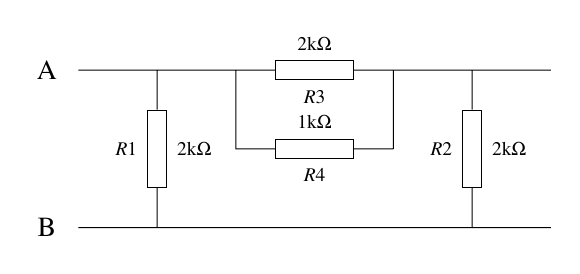
\begin{tikzpicture}[
    circuit ee IEC,
    x = 2cm, y = 1cm,
    every info/.style = {font = \scriptsize},
    set diode graphic = var diode IEC graphic,
    set make contact graphic = var make contact IEC graphic]

\draw (0,0) to (0.5,0) --
	  (0.5,0) to [resistor={ohm=2k, info'={$R1$}}] (0.5,-2) --
	  (0.5,-2) to (0, -2)
	  (0.5,0) to (1,0) --
	  (1,0) to [resistor={ohm=2k, info'={$R3$}}] (2,0)
	  (1,0) to (1,-1) --
	  (1,-1) to [resistor={ohm=1k, info'={$R4$}}] (2,-1)--
	  (2,-1) to (2,0) --
	  (2,0) to (2.5,0) --
	  (2.5,0) to [resistor={ohm=2k, info'={$R2$}}] (2.5, -2) --
	  (2.5,-2) to (3,-2)
	  (2.5,0) to (3,0) 
	  (0.5,-2) to (2.5,-2);
\path (-0.2,0) node(x) {{A}}
	  (-0.2,-2) node(x) {{B}};
\end{tikzpicture}
\end{figure}
\newline

Zadanie B, część II, obwód 6
\begin{figure}[!h]
\centering
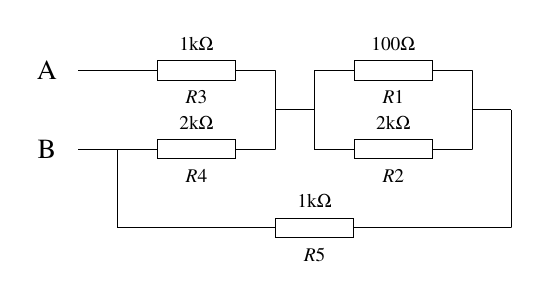
\begin{tikzpicture}[
    circuit ee IEC,
    x = 2cm, y = 1cm,
    every info/.style = {font = \scriptsize},
    set diode graphic = var diode IEC graphic,
    set make contact graphic = var make contact IEC graphic]

\draw (0,0) to (0.25,0) --
	  (0.25,0) to [resistor={ohm=1k, info'={$R3$}}] (1.25,0) --
	  (1.25,0) to (1.25, -0.5)
	  (0,-1) to (0.25,-1) --
	  (0.25,-1) to [resistor={ohm=2k, info'={$R4$}}] (1.25,-1)--
	  (1.25,-1) to (1.25,-0.5) --
	  (1.25,-0.5) to (1.5,-0.5) --
	  (1.5,-0.5) to (1.5,0) -- 
	  (1.5,0) to [resistor={ohm=100, info'={$R1$}}] (2.5,0)--
	  (2.5,0) to (2.5,-0.5)
	  (1.5,-0.5) to (1.5,-1) -- 
	  (1.5,-1) to [resistor={ohm=2k, info'={$R2$}}] (2.5,-1)--
	  (2.5,-1) to (2.5,-0.5)--
	  (2.5,-0.5) to (2.75, -0.5)
	  (0.25, -1) to (0.25, -2)--
	  (0.25, -2) to [resistor={ohm=1k, info'={$R5$}}] (2.75,-2)--
	  (2.75,-2) to (2.75,-0.5);
\path (-0.2,0) node(x) {{A}}
	  (-0.2,-1) node(x) {{B}};
\end{tikzpicture}
\end{figure}
\newline

Zadanie C, część II
\begin{figure}[!h]
\centering
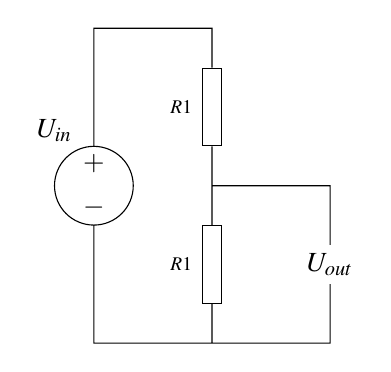
\begin{tikzpicture}[
    circuit ee IEC,
    x = 1cm, y = 1cm,
    every info/.style = {font = \scriptsize},
    set diode graphic = var diode IEC graphic,
    set make contact graphic = var make contact IEC graphic]

\draw (0,0) circle [radius = 0.5] 
	  (0,0.5) to (0,2) --
	  (0,2) to (1,2) --
	  (1.5,2) to [resistor={info'={$R1$}}] (1.5,0) --
	  (1.5,0) to [resistor={info'={$R1$}}] (1.5,-2) --
	  (1.5,-2) to (0,-2) --
	  (0,-2) to (0,-0.5)
	  (1.5,0) to  (3,0) -- 
	  (3,0) to (3,-0.75)
	  (1.5,-2) to (3,-2) --
	  (3,-2) to (3,-1.25) 
	  ;
\path (-0.5,0.7) node(x) {{$U_{in}$}}
	  (0,0.28) node(x) {{$\Large +$}}
	  (0,-0.28) node(x) {{$\Large -$}}
	  (3,-1) node(x) {{$U_{out}$}}
	  ;
\end{tikzpicture}
\end{figure}
\newpage

Zadanie C, część III
\begin{figure}[!h]
\centering
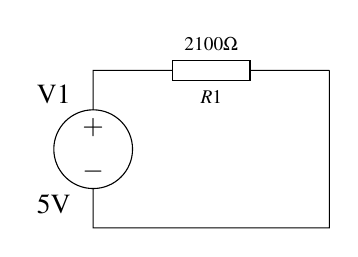
\begin{tikzpicture}[
    circuit ee IEC,
    x = 1cm, y = 1cm,
    every info/.style = {font = \scriptsize},
    set diode graphic = var diode IEC graphic,
    set make contact graphic = var make contact IEC graphic]

\draw (0,0) circle [radius = 0.5] 
	  (0,0.5) to (0,1) --
	  (0,1) to [resistor={ohm = 2100, info'={$R1$}}] (3,1) --
	  (3,1) to (3,-1) -- 
	  (3,-1) to (0,-1) --
	  (0,-1) to (0,-0.5);
\path (-0.5,0.7) node(x) {{V1}}
	  (-0.5,-0.7) node(x) {{5V}}
	  (0,-0.28) node(x) {{$\Large -$}}
	  (0,0.28) node(x) {{$\Large +$}}
	  ;
\end{tikzpicture}
\end{figure}
\newline

Zadanie C, część IV, obwód 1
\begin{figure}[!h]
\centering
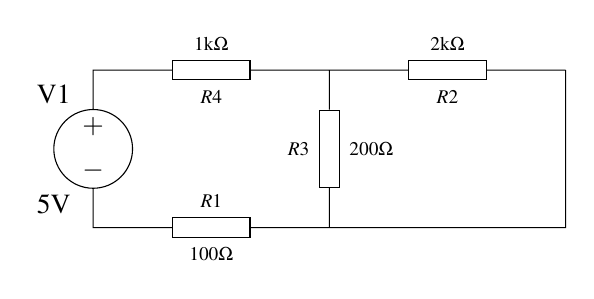
\begin{tikzpicture}[
    circuit ee IEC,
    x = 1cm, y = 1cm,
    every info/.style = {font = \scriptsize},
    set diode graphic = var diode IEC graphic,
    set make contact graphic = var make contact IEC graphic]

\draw (0,0) circle [radius = 0.5] 
	  (0,0.5) to (0,1) --
	  (0,1) to [resistor={ohm = 1k, info'={$R4$}}] (3,1) --
	  (3,1) to [resistor={ohm = 200, info'={$R3$}}](3,-1) -- 
	  (3,-1) to [resistor={ohm = 100, info'={$R1$}}](0,-1) --
	  (0,-1) to (0,-0.5)
	  (3,1) to [resistor={ohm = 2k, info'={$R2$}}] (6,1) --
	  (6,1) to (6,-1) --
	  (6,-1) to (3,-1);
\path (-0.5,0.7) node(x) {{V1}}
	  (-0.5,-0.7) node(x) {{5V}}
	  (0,-0.28) node(x) {{$\Large -$}}
	  (0,0.28) node(x) {{$\Large +$}}
	  ;
\end{tikzpicture}
\end{figure}
\newline

\bibliography{IEEEabrv,refs}

\end{document}

